\documentclass{article}
\usepackage{graphicx} % Required for inserting images
\usepackage{minted}
\usepackage{array}

\title{Circuitos Digitais I - Atividades 1-3: Aulas 4-5}
\author{Luis Felipe Ferreira Soares}
\date{Outubro 2025}

\begin{document}

\maketitle

\setcounter{section}{1}
\setcounter{subsection}{0}
\section*{Atividade 1}
\subsection{Conversor BCD8421 para Excesso de 3}
\begin{minted}{verilog}
module bcd2xs3 (
    input [3:0] bcd,
    output [3:0] xs3
);

reg [3:0] xs3_reg;

always @(*) begin
    case (bcd)
    4'b0000: xs3_reg = 4'b0011;
    4'b0001: xs3_reg = 4'b0100;
    4'b0010: xs3_reg = 4'b0101;
    4'b0011: xs3_reg = 4'b0110;
    4'b0100: xs3_reg = 4'b0111;
    4'b0101: xs3_reg = 4'b1000;
    4'b0110: xs3_reg = 4'b1001;
    4'b0111: xs3_reg = 4'b1010;
    4'b1000: xs3_reg = 4'b1011;
    4'b1001: xs3_reg = 4'b1100;
    default: xs3_reg = 4'b0000;
    endcase
end

assign xs3 = xs3_reg;

endmodule
\end{minted}

\newpage

\subsection{Testbench}
\begin{minted}{verilog}
module bcd2xs3_tb;
reg [3:0] bcd;
wire [3:0] xs3;

bcd2xs3 dut (bcd, xs3);

initial begin
    $display("DCBA | WXYZ");
    $monitor("%4b | %4b", bcd, xs3);
    bcd = 4'b0000; #10;
    bcd = 4'b0001; #10;
    bcd = 4'b0010; #10;
    bcd = 4'b0011; #10;
    bcd = 4'b0100; #10;
    bcd = 4'b0101; #10;
    bcd = 4'b0110; #10;
    bcd = 4'b0111; #10;
    bcd = 4'b1000; #10;
    bcd = 4'b1001; #10;
end

endmodule
\end{minted}

\subsection{Console Output}
\begin{verbatim}
DCBA | WXYZ
0000 | 0011
0001 | 0100
0010 | 0101
0011 | 0110
0100 | 0111
0101 | 1000
0110 | 1001
0111 | 1010
1000 | 1011
1001 | 1100
\end{verbatim}

\subsection{Portas lógicas do Conversor}
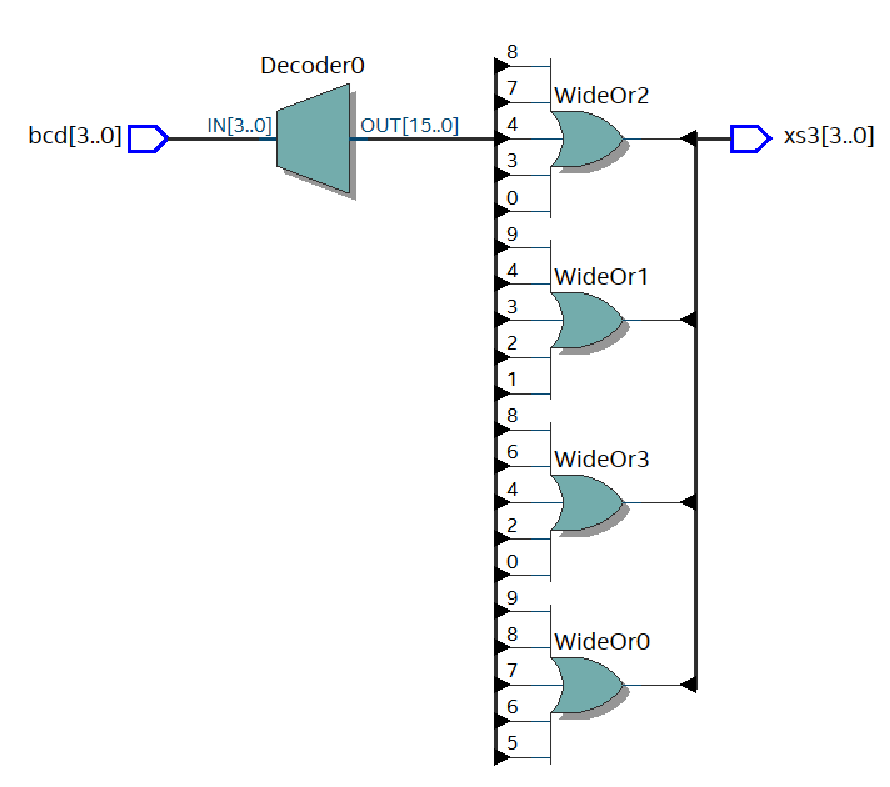
\includegraphics[width=1\textwidth]{bcd2xs3-comportamental-rtl.png}

\subsection{Simulação}
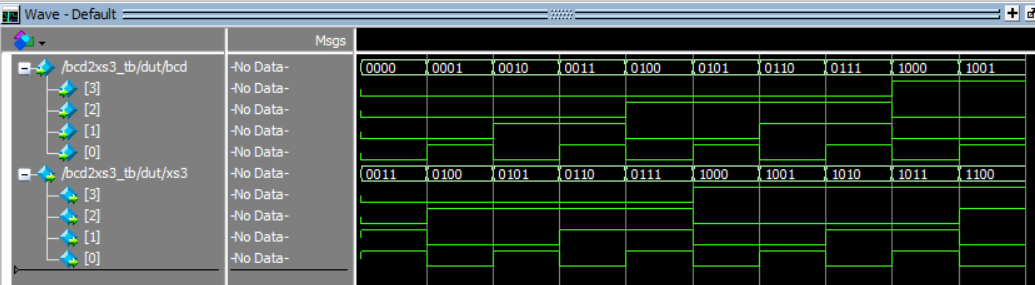
\includegraphics[width=1\textwidth]{bcd2xs3-comportamental-wave.png}

\newpage

\setcounter{section}{2}
\setcounter{subsection}{0}
\section*{Atividade 2}

\subsection{Conversor BCD8421 para Código Gray}
\begin{minted}{verilog}
module dcba2gray (
    input [3:0] bcd,
    output reg [3:0] gray
);

always @(*)
begin
  case (bcd)
    4'b0000: gray = 4'b0000;
    4'b0001: gray = 4'b0001;
    4'b0010: gray = 4'b0011;
    4'b0011: gray = 4'b0010;
    4'b0100: gray = 4'b0110;
    4'b0101: gray = 4'b0111;
    4'b0110: gray = 4'b0101;
    4'b0111: gray = 4'b0100;
    4'b1000: gray = 4'b1100;
    4'b1001: gray = 4'b1101;
    4'b1010: gray = 4'b1111;
    4'b1011: gray = 4'b1110;
    4'b1100: gray = 4'b1010;
    4'b1101: gray = 4'b1011;
    4'b1110: gray = 4'b1001;
    4'b1111: gray = 4'b1000;
    default: gray = 4'bxxxx;
  endcase
end

endmodule
\end{minted}

\newpage

\subsection{Testbench}
\begin{minted}{verilog}
module dcba2gray_tb;
reg [3:0] bcd;
wire [3:0] gray;


always #1 bcd[0] = !bcd[0];
always #2 bcd[1] = !bcd[1];
always #4 bcd[2] = !bcd[2];
always #8 bcd[3] = !bcd[3];

dcba2gray dut(bcd, gray);

initial begin
    $display("DCBA | WXYZ");
    $monitor("%4b | %4b", bcd, gray);
    bcd = 4'b0000;
    #16 $finish;
end

endmodule
\end{minted}

\subsection{Console output}
\begin{verbatim}
DCBA | WXYZ
0000 | 0000
0001 | 0001
0010 | 0011
0011 | 0010
0100 | 0110
0101 | 0111
0110 | 0101
0111 | 0100
1000 | 1100
1001 | 1101
1010 | 1111
1011 | 1110
1100 | 1010
1101 | 1011
1110 | 1001
1111 | 1000
\end{verbatim}

\subsection{Portas lógicas}
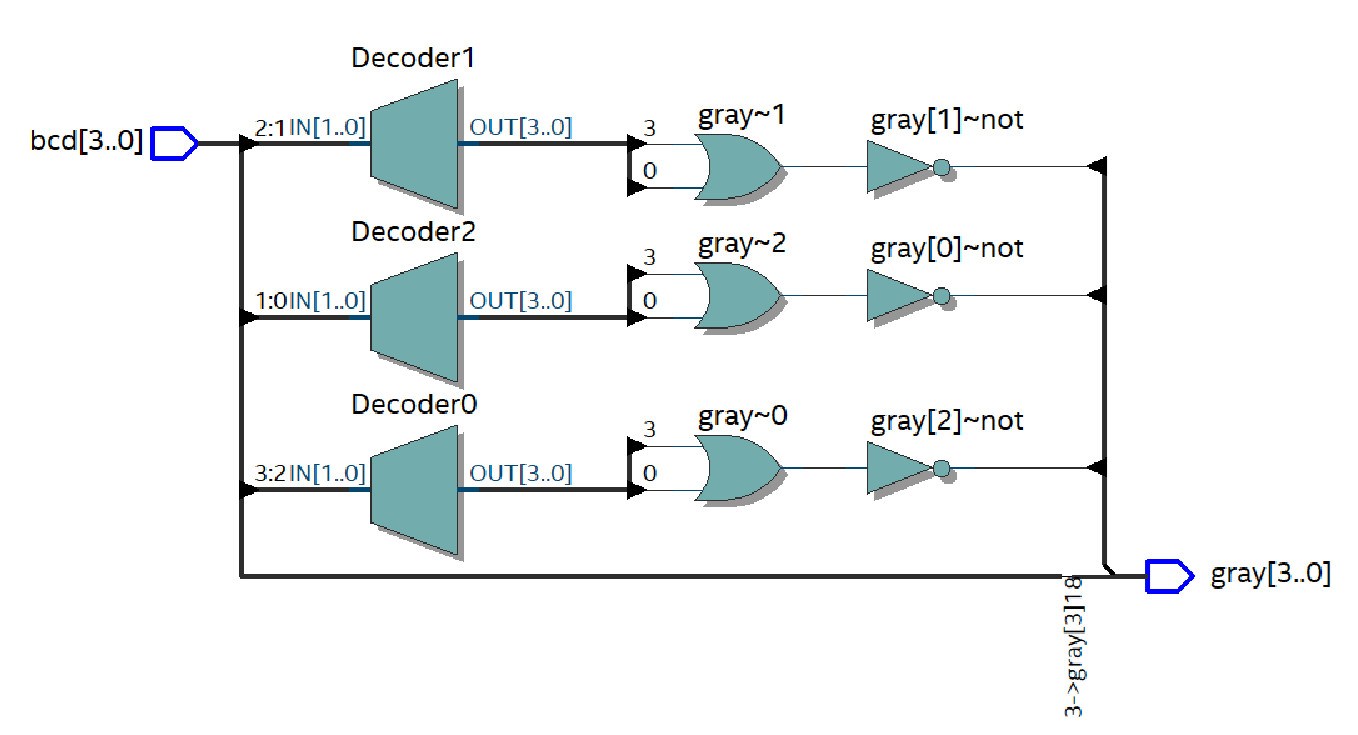
\includegraphics[width=1\textwidth]{bcd2gray-comportamental-rtl.png}

\subsection{Simulação}
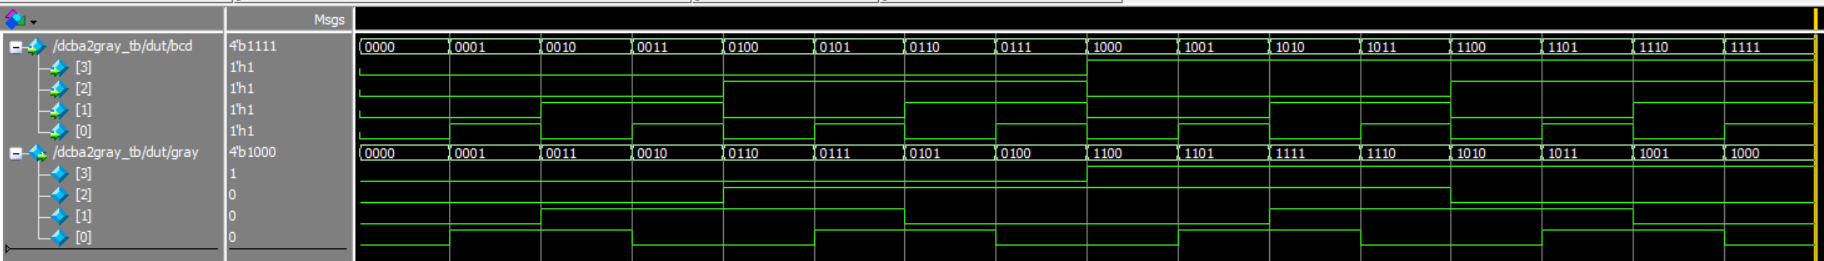
\includegraphics[width=1\textwidth]{bcd2gray-comportamental-wave.png}

\newpage

\setcounter{section}{3}
\setcounter{subsection}{0}
\section*{Atividade 3}

\subsection{Conversor BCD8421 para 7-Segmentos (Extendido)}
\begin{minted}{verilog}
module dcba27segments (
    input [3:0] dcba,
    output reg [6:0] segments 
);

always @ (*) begin
    case (dcba)
        4'b0000: segments = 7'b0000001;
        4'b0001: segments = 7'b1001111;
        4'b0010: segments = 7'b0010010;
        4'b0011: segments = 7'b0000110;
        4'b0100: segments = 7'b1001100;
        4'b0101: segments = 7'b0100100;
        4'b0110: segments = 7'b0100000;
        4'b0111: segments = 7'b0001111;
        4'b1000: segments = 7'b0000000;
        4'b1001: segments = 7'b0000100;
        4'b1010: segments = 7'b0001000; // A
        4'b1011: segments = 7'b1100000; // b
        4'b1100: segments = 7'b0110001; // C
        4'b1101: segments = 7'b1000010; // d
        4'b1110: segments = 7'b0110000; // E
        4'b1111: segments = 7'b0111000; // F
        default: segments = 7'b1111111;
    endcase
end

endmodule
\end{minted}

\newpage

\subsection{Testbench}
\begin{minted}{verilog}
module dcba27segments_tb;
reg [3:0] dcba;
wire [6:0] segments;

dcba27segments dut (dcba, segments);

always #1 dcba[0] = !dcba[0];
always #2 dcba[1] = !dcba[1];
always #4 dcba[2] = !dcba[2];
always #8 dcba[3] = !dcba[3];

initial begin
    $display("DCBA | SEGMENT");
    $monitor("%b | %b", dcba, segments);
    dcba = 4'b0000;
    #16 $finish;
end

endmodule
\end{minted}

\subsection{Console output}
\begin{verbatim}
DCBA | SEGMENT
0000 | 0000001
0001 | 1001111
0010 | 0010010
0011 | 0000110
0100 | 1001100
0101 | 0100100
0110 | 0100000
0111 | 0001111
1000 | 0000000
1001 | 0000100
1010 | 0001000
1011 | 1100000
1100 | 0110001
1101 | 1000010
1110 | 0110000
1111 | 0111000
\end{verbatim}

\subsection{Portas lógicas}
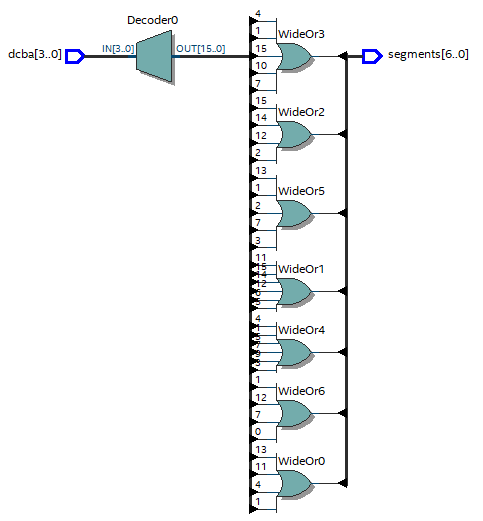
\includegraphics[width=1\textwidth]{dcba27segments-rtl.png}

\subsection{Simulação}
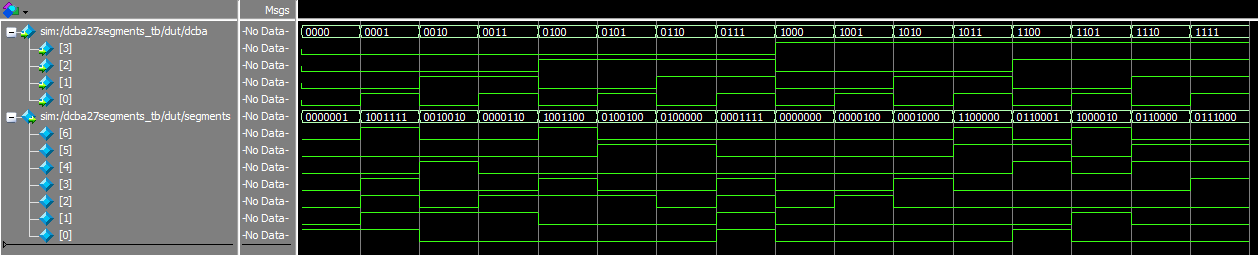
\includegraphics[width=1\textwidth]{dcba27segments-wave.png}

\end{document}